\documentclass{article}

% Language setting
% Replace `english' with e.g. `spanish' to change the document language
\usepackage[czech]{babel}

% Set page size and margins
% Replace `letterpaper' with `a4paper' for UK/EU standard size
\usepackage[a4paper,top=2cm,bottom=2cm,left=3cm,right=3cm,marginparwidth=1.75cm]{geometry}

% Useful packages
\usepackage{amsmath}
\usepackage{graphicx}
\usepackage{tikz}
\usetikzlibrary{automata}
\usetikzlibrary{positioning}
\usetikzlibrary{arrows.meta}
\usepackage[colorlinks=true, allcolors=blue]{hyperref}

\tikzset{
node distance=5cm, % Minimum distance between two nodes. Change this if you need to.
every state/.append style={ % Sets the style of each state
semithick,
% fill=gray!10 % Shade nodes
},
initial/.append style={
initial text={}, % No label on start arrow
initial distance=0.5cm % Lengthen the initial arrow
},
accepting/.append style={ % Set the style of each accepting state
% double=gray!10, % Shade space between inner and outer circles
double distance=2pt, % Space between inner and outer circles
outer sep=1pt % Shorten arrows by half of double distance
},
every edge/.append style={ % Sets the properties for each transition
draw,
->,>=Stealth,  % Makes edges directed with bold arrowheads
auto, % Put edge labels to the left
semithick
}
}
\let\epsilon\varepsilon
\let\sym\texttt

\title{\textbf{INC Projekt -- Výstupní zpráva}}
\author{Tomáš Kolařík (xkolart01)}

\begin{document}
\maketitle

\section{Architektura navrženého obvodu (na úrovni RTL)}

\subsection{Schéma obvodu}

\begin{figure}[h]
    \centering
    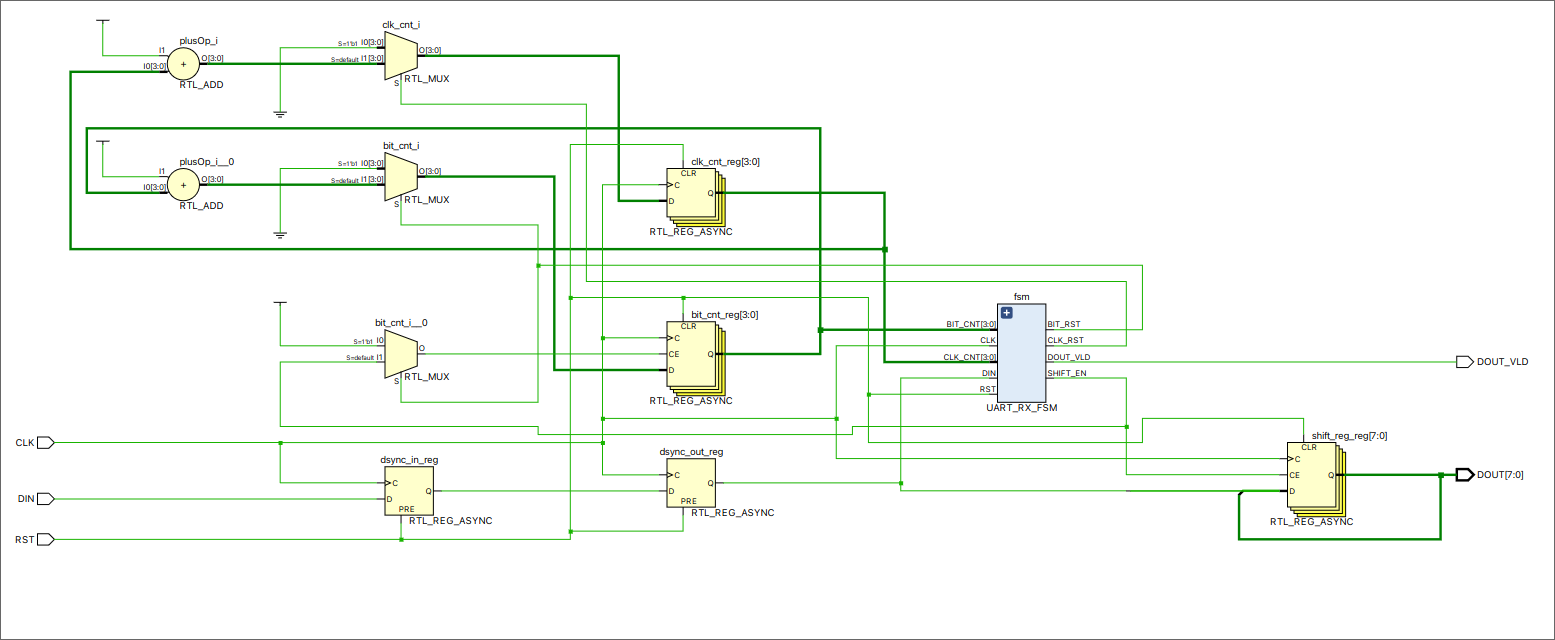
\includegraphics[width=\linewidth]{schematic}
\end{figure}

\subsection{Popis funkce}
Obvod se skládá z 5 hlavních částí:
\begin{enumerate}
    \item \textbf{Synchronizačního obvodu}, který omezuje pravděpodobnost vzniku metastabilních stavů asynchronního vstupu \textit{DIN} (projde 2 klopnými obvody \textit{dsync\_in\_reg} a \textit{dsync\_out\_reg}, potom se používá jako obyčejný \textit{DIN} ve zbytku obvodu),
    \item \textbf{Čítače pulsů hodinového signálu \textit{CLK} \textit{(clk\_cnt\_reg)}}, jehož pomocí můžeme vzorkovat příchozí bity přímo uprostřed nich (v midbitu) a také je součástí podmínek FSM pro přechod do jiných stavů,
    \item \textbf{Čítače příchozích bitů \textit{(bit\_cnt\_reg)}}, který je součástí podmínek FSM pro přechod do jiných stavů (specificky ze stavu \textit{DATA} $\rightarrow$ \textit{STOP}),
    \item \textbf{Posuvného registru výstupu \textit{DOUT} \textit{(shift\_reg\_reg)}}, kam se postupně přidávají hodnoty příchozích bitů z \textit{DIN},
    \item \textbf{Obvodu konečného automatu \textit{(FSM)}}, více vysvětleného níže.
\end{enumerate}

\section{Návrh automatu (Finite State Machine)}

\subsection{Schéma automatu}
\begin{tikzpicture}
\node[state, initial] (idle) at (0,0)  {$\text{IDLE}$};
\node[state] (start) at (3, 3)  {$\text{START}$};
\node[state] (data) at (6, 0)  {$\text{DATA}$};
\node[state] (stop) at (3, -3)  {$\text{STOP}$};
\draw (idle) edge[loop right] node {
    \sym{else / --}
} (idle);
\draw (idle) edge node {
    \sym{DIN = 0 / CLK\_RST, BIT\_RST}
} (start);
\draw (start) edge[loop above] node {
    \sym{else / --}
} (start);
\draw (start) edge node {
    \sym{CLK\_CNT = 7 / CLK\_RST}
} (data);
\draw (data) edge[loop right] node {
    \sym{CLK\_CNT = 15 / CLK\_RST, SHIFT\_EN}
} (data);
\draw (data) edge node {
    \sym{BIT\_CNT = 8 / BIT\_RST, DOUT\_VLD}
} (stop);
\draw (stop) edge[loop below] node {
    \sym{else / --}
} (stop);
\draw (stop) edge node {
    \sym{CLK\_CNT = 15 / CLK\_RST}
} (idle);
\end{tikzpicture}

\\

\begin{itemize}
    \item \textbf{Stavy automatu}: \textit{IDLE}, \textit{START}, \textit{DATA}, \textit{STOP}
    \item \textbf{Vstupní signály}: \textit{DIN}, \textit{CLK\_CNT}, \textit{BIT\_CNT}
    \item \textbf{Moorovy výstupy}: žádné
    \item \textbf{Mealyho výstupy}: \textit{CLK\_RST}, \textit{BIT\_RST}, \textit{SHIFT\_EN}, \textit{DOUT\_VLD}
\end{itemize}

\subsection{Popis funkce}
Počáteční stav automatu je \textbf{IDLE}. Automat čeká na start bit, tedy na log. 0 na \textit{DIN} (UART idluje v log. 1). Po zjištění start bitu se přesune do stavu \textbf{START} a zresetuje počítadla pulsů \textit{CLK} (\textit{CLK\_CNT}) a příchozích bitů (\textit{BIT\_CNT}) pomocí signálů \textit{CLK\_RST} a \textit{BIT\_RST}. Ve stavu \textbf{START} automat čeká na 7. takt signálu \textit{CLK}, což signalizuje, že jsme přibližně uprostřed start bitu. Potom přejde do stavu \textbf{DATA} a mezitím vyšle signál \textit{CLK\_RST}, čímž zresetuje počítadlo pulsů \textit{CLK}. Tím se zajistí, že všechny následující datové bity budou vzorkovány přibližně uprostřed svých bitů. Po dosažení hodnoty \textit{CLK\_CNT = 15} automat vyšle signály \textit{CLK\_RST}, čímž znovu zresetuje počítadlo pro další bit, a \textit{SHIFT\_EN}, čímž automat signalizuje posuvnému registru, aby načetl příchozí bit. Po přečtení všech 8 bitů přejde automat do stavu \textbf{STOP} a vyšle signály \textit{BIT\_RST}, čímž zresetuje počítadlo příchozích bitů, a \textit{DOUT\_VLD}, čímž potvrdí, že výsledek \textit{DOUT} z posuvného registru je platný. Po dosažení hodnoty \textit{CLK\_CNT = 15} se automat vrací zpět do stavu \textbf{IDLE} a vysílá signál \textit{CLK\_RST}, čímž se vrací do počátečního stavu.

\newpage

\section{Snímek obrazovky ze simulací}

\begin{figure}[h]
    \centering
    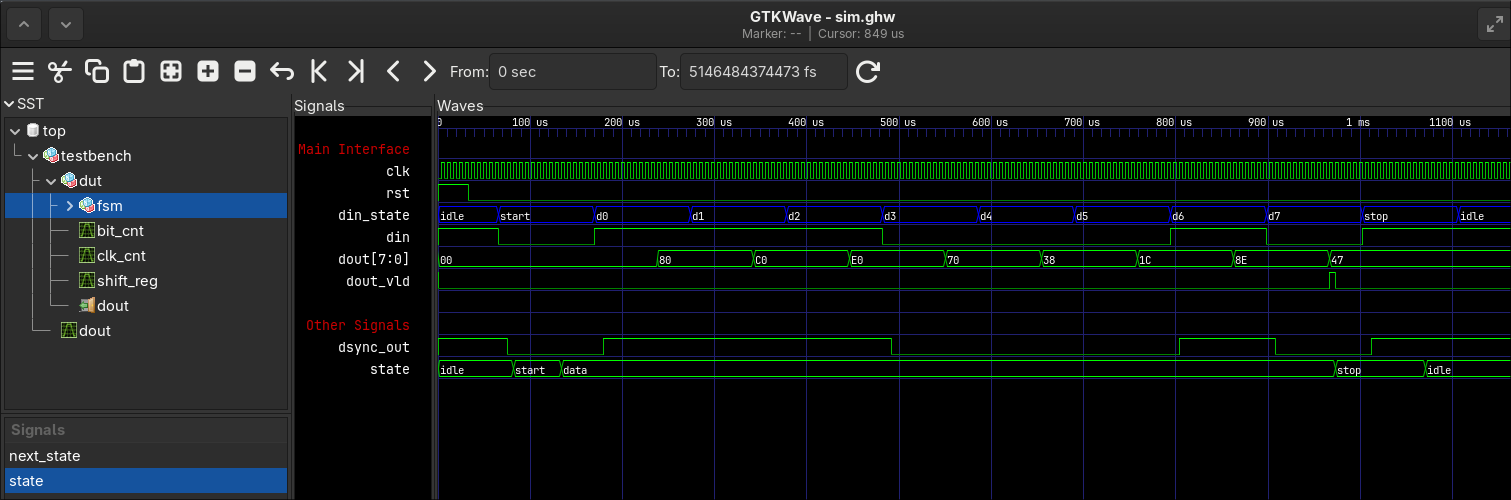
\includegraphics[width=\linewidth]{simulation}
\end{figure}

\end{document}
